\documentclass{beamer}

% Theme selection
\usetheme{Madrid}
\usecolortheme{beaver}

% Packages
\usepackage{graphicx}
\usepackage{booktabs}
\usepackage{tikz}

% Title Information
\title{Unit 1: Basic Economic Concepts}
\subtitle{}
\author{Doğukan Günkördü}
\date{}

\begin{document}

% Title Slide
\begin{frame}
    \titlepage
\end{frame}

% Table of Contents
\begin{frame}{Unit 1 Roadmap}
    \tableofcontents
\end{frame}

% SECTION 1: INTRODUCTION TO ECONOMICS
\section{The Discipline of Economics}

\begin{frame}{What is Economics?}
    \begin{block}{Definition}
        Economics is the social science that studies how resources are used and is concerned with how resources can be used to their fullest potential.
    \end{block}
    
    \begin{itemize}
        \item \textbf{The Core Problem:} \alert{Scarcity}.
        \item We have unlimited wants but limited resources.
        \item \textbf{Microeconomics:} Focuses on individual units (families, firms, individuals).
        \item \textbf{Macroeconomics:} Focuses on the economy as a whole (inflation, unemployment, GDP).
    \end{itemize}
\end{frame}

\begin{frame}{Positive vs. Normative Economics}
    \begin{itemize}
        \item \textbf{Positive Economics:}
        \begin{itemize}
            \item Based on the scientific method.
            \item Hypotheses are formulated and tested.
            \item \textit{Example:} "If the price of gas rises, people will buy less gas." (Fact-based).
        \end{itemize}
        \vspace{0.5cm}
        \item \textbf{Normative Economics:}
        \begin{itemize}
            \item Based on value judgments and opinions.
            \item Describes how things \textit{ought} to be.
            \item \textit{Example:} "We should spend more on education than defense."
        \end{itemize}
    \end{itemize}
\end{frame}

% SECTION 2: RESOURCES AND OPPORTUNITY COST
\section{Resources and Opportunity Cost}

\begin{frame}{Factors of Production (Resources)}
    Economists classify resources into three main categories (sometimes four):
    
    \begin{enumerate}
        \item \textbf{Land:} All natural resources (timber, oil, oceans, minerals).
        \item \textbf{Labor:} Human attributes that are productive (physical work, intellectual capabilities).
        \item \textbf{Capital:} Productive equipment or machinery used to produce other goods (factories, computers, forklifts).
        \item \textit{(Entrepreneurship): Risk-taking and organization of resources.}
    \end{enumerate}
\end{frame}

\begin{frame}{Opportunity Cost}
    \begin{block}{Definition}
        Opportunity cost is what must be sacrificed to obtain something. It is the value of the \textbf{next best alternative} foregone.
    \end{block}

    \begin{exampleblock}{Real World Examples}
        \begin{itemize}
            \item \textbf{Student's Time:} Spending 2 hours studying means sacrificing 2 hours of TV or socializing.
            \item \textbf{College:} The cost isn't just tuition; it is the \textit{lost wages} you could have earned by working instead.
        \end{itemize}
    \end{exampleblock}
\end{frame}

% SECTION 3: PRODUCTION POSSIBILITIES FRONTIER
\section{Production Possibilities Frontier (PPF)}

\begin{frame}{Production Possibilities Frontier (PPF)}
    The PPF is a graph showing the combinations of two goods an economy can produce if it uses all resources \textbf{fully and efficiently}.
    
    \begin{columns}
        \column{0.5\textwidth}
        \textbf{Key Concepts:}
        \begin{itemize}
            \item \textbf{Points on the curve:} Efficient.
            \item \textbf{Points inside the curve:} Inefficient (unemployment).
            \item \textbf{Points outside the curve:} Unobtainable with current resources.
        \end{itemize}
        
        \column{0.5\textwidth}
        \begin{center}
        % Simple TikZ graph for PPF
        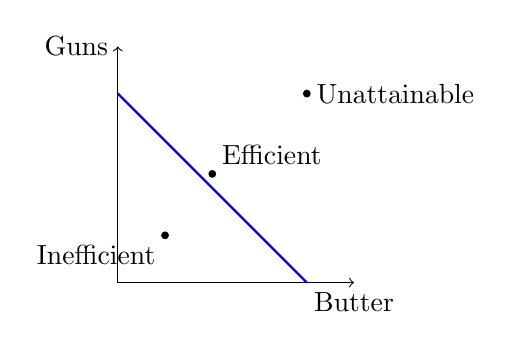
\begin{tikzpicture}[scale=0.6]
            \draw[<->] (0,5) node[left]{Guns} -- (0,0) -- (5,0) node[below]{Butter};
            \draw[thick, blue] (0,4) to[out=-45,in=135] (4,0);
            \filldraw (2,2.3) circle (2pt) node[above right]{Efficient};
            \filldraw (1,1) circle (2pt) node[below left]{Inefficient};
            \filldraw (4,4) circle (2pt) node[right]{Unattainable};
        \end{tikzpicture}
        \end{center}
    \end{columns}
\end{frame}

\begin{frame}{Law of Increasing Opportunity Costs}
    \begin{itemize}
        \item Why is the PPF usually bowed out (concave to the origin)?
        \item \textbf{The Law of Increasing Costs:} As more of a product is produced, the opportunity cost increases.
        \item \textbf{Reason:} Resources are not perfectly adaptable.
        \begin{itemize}
            \item \textit{Example:} Farmers and cows are good at making butter, not guns. Shifting them to gun production results in a large loss of butter for a small gain in guns.
        \end{itemize}
        \item \textit{Note: If opportunity costs are constant, the PPF is a straight line.}
    \end{itemize}
\end{frame}

\begin{frame}{Shifting the PPF}
    Two factors cause the PPF to shift:
    \begin{enumerate}
        \item \textbf{Change in Quantity/Quality of Resources:} 
        \begin{itemize}
            \item Population growth, new territories, more capital.
        \end{itemize}
        \item \textbf{Change in Technology:} 
        \begin{itemize}
            \item Robotics, AI, better farming methods.
        \end{itemize}
    \end{enumerate}
    
    \begin{alertblock}{Important Note}
        A decline in unemployment moves the economy from a point \textit{inside} the curve to a point \textit{on} the curve. It does \textbf{not} shift the curve.
    \end{alertblock}
\end{frame}

% SECTION 4: COMPARATIVE ADVANTAGE
\section{Comparative Advantage and Trade}

\begin{frame}{Absolute vs. Comparative Advantage}
    \begin{itemize}
        \item \textbf{Absolute Advantage:} A nation can produce a product more efficiently (with fewer inputs) than another nation.
        \item \textbf{Comparative Advantage:} A nation can produce a good at a \textbf{lower opportunity cost} than another nation.
    \end{itemize}
    
    \begin{block}{The Law of Comparative Advantage (Ricardo)}
        Nations should specialize in producing goods where they have a comparative advantage and trade for the rest. This increases total output.
    \end{block}
\end{frame}

\begin{frame}{Calculating Opportunity Cost (Input Problem)}
    \textit{Example from Barron's: Labor Hours Needed (Input)}
    
    \begin{table}[]
        \begin{tabular}{lcc}
            \toprule
            Country & Wheat & Cloth \\
            \midrule
            Portugal & 10 hours & 20 hours \\
            England & 20 hours & 60 hours \\
            \bottomrule
        \end{tabular}
    \end{table}

    \textbf{Calculations:}
    \begin{itemize}
        \item \textbf{Portugal:} 
            \begin{itemize}
                \item Cost of 1 Wheat = $10/20 = 0.5$ Cloth.
                \item Cost of 1 Cloth = $20/10 = 2$ Wheat.
            \end{itemize}
        \item \textbf{England:} 
            \begin{itemize}
                \item Cost of 1 Wheat = $20/60 = 0.33$ Cloth.
                \item Cost of 1 Cloth = $60/20 = 3$ Wheat.
            \end{itemize}
    \end{itemize}
    \footnotesize{Result: England has comp. advantage in Wheat (0.33 < 0.5). Portugal has comp. advantage in Cloth (2 < 3).}
\end{frame}

% SECTION 5: ECONOMIC SYSTEMS
\section{Economic Systems}

\begin{frame}{Fundamental Economic Questions}
    Every economy must answer three questions due to scarcity:
    
    \begin{enumerate}
        \item \textbf{What} should be produced?
        \item \textbf{How} much should be produced?
        \item \textbf{For Whom} (Who gets what)?
    \end{enumerate}
\end{frame}

\begin{frame}{Comparing Economic Systems}
    \begin{columns}
        \column{0.5\textwidth}
        \textbf{Command Economy}
        \begin{itemize}
            \item Central government dictates production and distribution.
            \item Prices/Wages set by government.
            \item \textit{Pros:} Can ensure equity, address social goals.
            \item \textit{Cons:} Inefficient, lack of incentives, shortages/surpluses.
            \item \textit{Ex:} North Korea, Cuba.
        \end{itemize}
        
        \column{0.5\textwidth}
        \textbf{Capitalism (Market Economy)}
        \begin{itemize}
            \item Supply and demand determine prices.
            \item Decentralized decision making.
            \item \textbf{Allocative Efficiency:} Resources go where society values them most.
            \item \textbf{The Invisible Hand:} Self-interest leads to societal benefit (Adam Smith).
        \end{itemize}
    \end{columns}
\end{frame}


\begin{frame}{Command vs. Market Economy: Evidence}
    \begin{figure}
        \centering
        % Change 'korea.jpg' to the exact name of your file
        \includegraphics[width=0.475\textwidth]{korea.jpg}
        \caption{North Korea (Command) vs. South Korea (Market) at Night}
    \end{figure}
\end{frame}






\begin{frame}{The Circular Flow Diagram}
    Shows the flow of resources, products, and money in a market economy.
    
    \begin{itemize}
        \item \textbf{Households:} Own resources (Land, Labor, Capital). Sell resources to firms; buy goods.
        \item \textbf{Firms:} Buy resources; produce and sell goods.
        \item \textbf{Resource Market (Factor Market):} Where labor/capital are sold. Households = Sellers, Firms = Buyers.
        \item \textbf{Product Market:} Where goods/services are sold. Firms = Sellers, Households = Buyers.
    \end{itemize}
\end{frame}

\begin{frame}{Summary of Unit 1}
    \begin{itemize}
        \item Economics is the study of scarcity.
        \item Opportunity cost is the value of the next best alternative.
        \item The PPF shows efficiency and opportunity cost; bowed shape = increasing costs.
        \item Trade is based on Comparative Advantage (lowest opportunity cost).
        \item Market economies rely on prices and self-interest to achieve allocative efficiency.
    \end{itemize}
\end{frame}

\end{document}
